% Slides for 2024-07-02
% To create a slide, use the following:
% \begin{frame}{TITLE}
%     BODY
% \end{frame}



\begin{frame}{Terraform and CI/CD}
    \begin{columns}
        \begin{column}{0.5\textwidth}
            Provisioning \\
            Docker Image
        \end{column}
        \begin{column}{0.5\textwidth}
            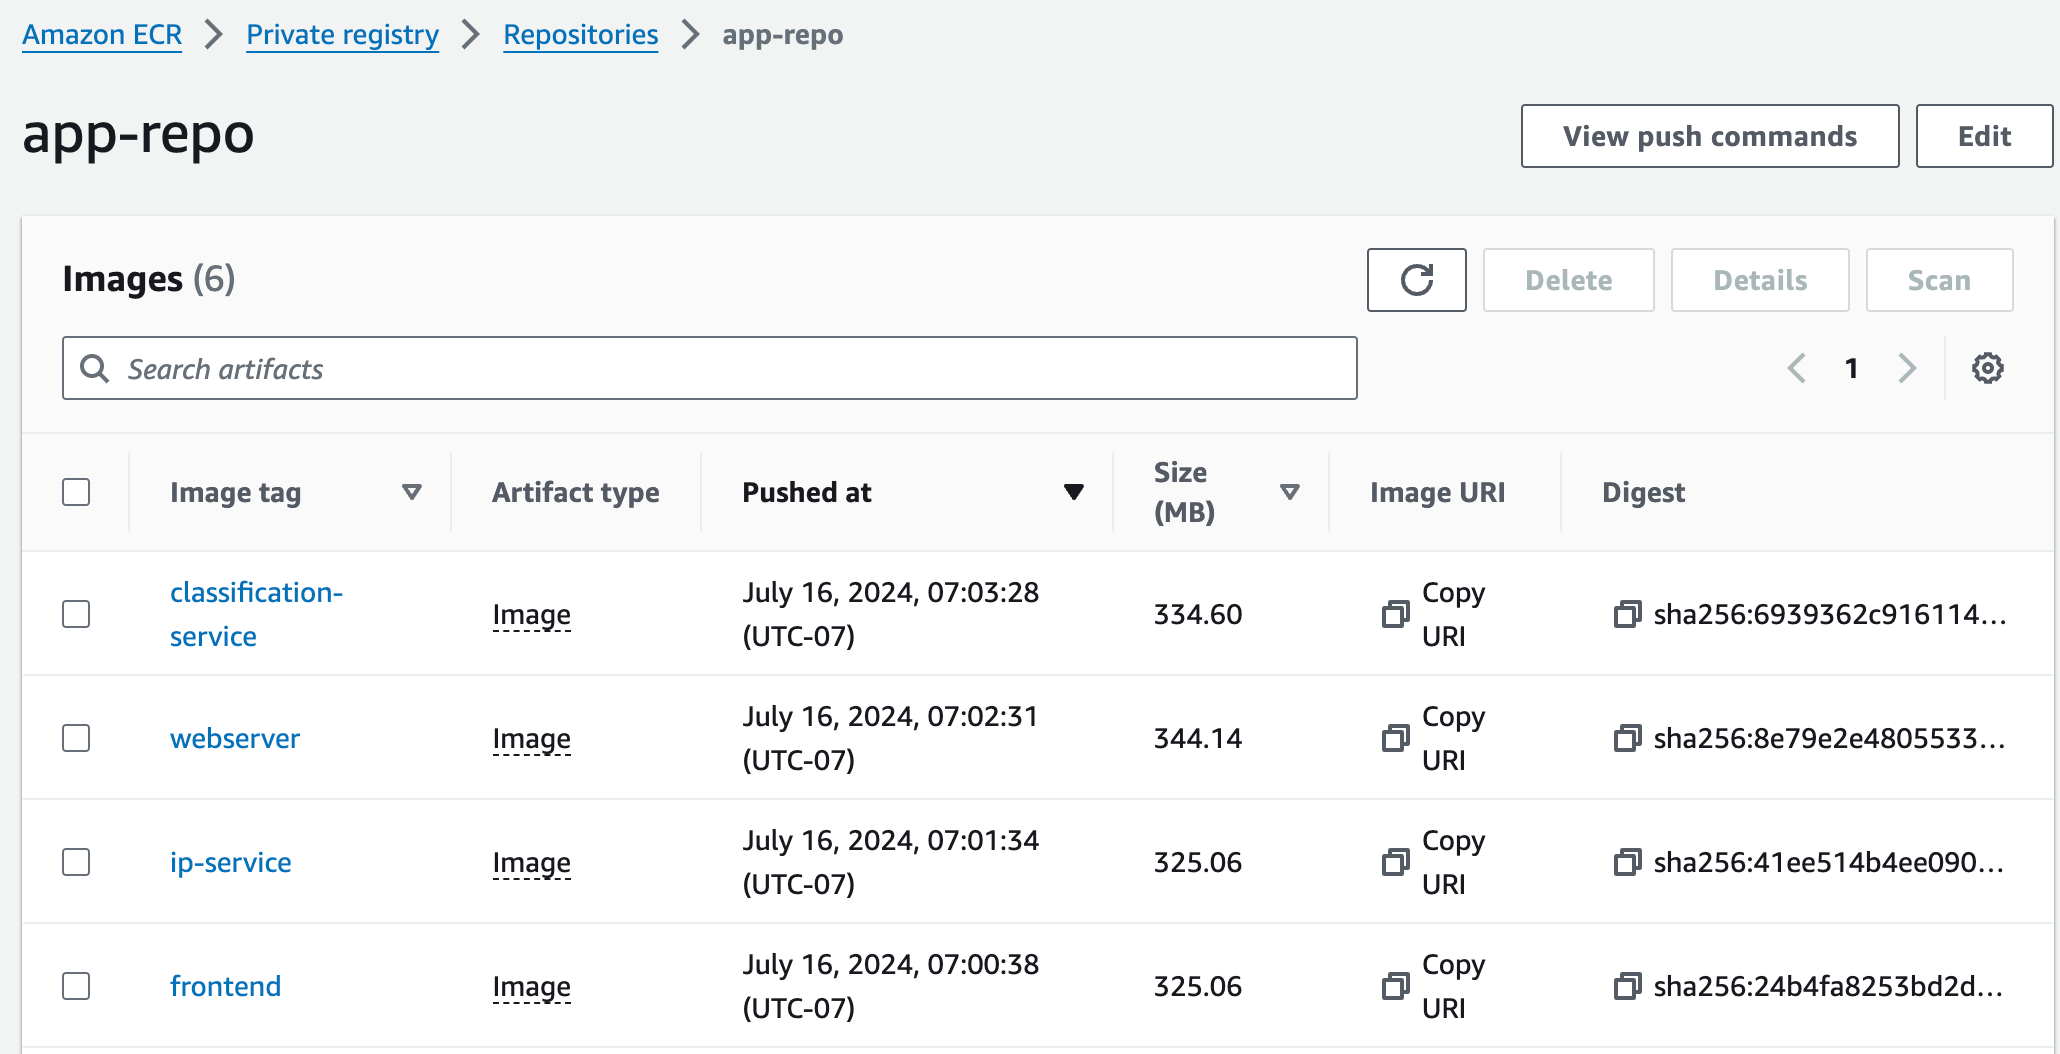
\includegraphics[height=0.7\textheight,width=0.7\textwidth,keepaspectratio]{images/mm_ecr.png} 
        \end{column}
    \end{columns}
\end{frame}



\begin{frame}{Auth0 Updates}
    \centering
    
\includegraphics[height=0.7\textheight,width=0.7\textwidth,keepaspectratio]{images/mm_auth0.png}
    Moving to Google OAuth 2.0
\end{frame}

% \begin{frame}{Infrastructure as Code AWS}
%     \centering
%     \includegraphics[height=0.6\textheight,width=0.6\textwidth,keepaspectratio]{images/mm_terraform.png}
% \end{frame}



\begin{frame}{Foundational Classification Model}
    \centering
    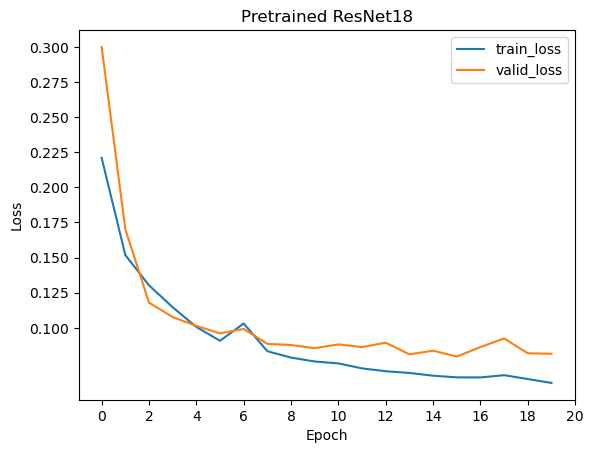
\includegraphics[height=0.6\textheight,width=0.6\textwidth,keepaspectratio]{images/pretrained.png}
    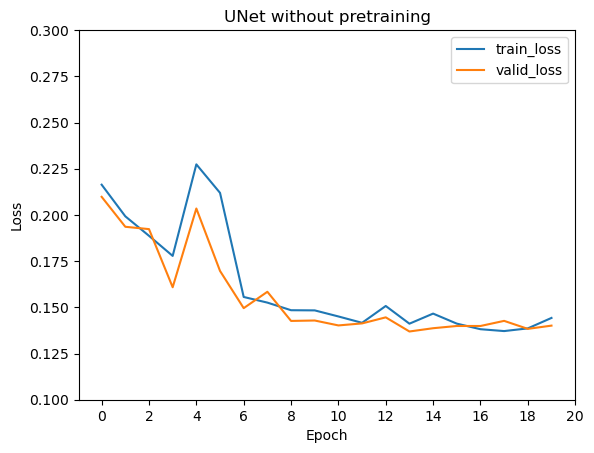
\includegraphics[height=0.6\textheight,width=0.6\textwidth,keepaspectratio]{images/untrained.png}
\end{frame}

\begin{frame}{Super Resolution Pipeline}
    \centering
    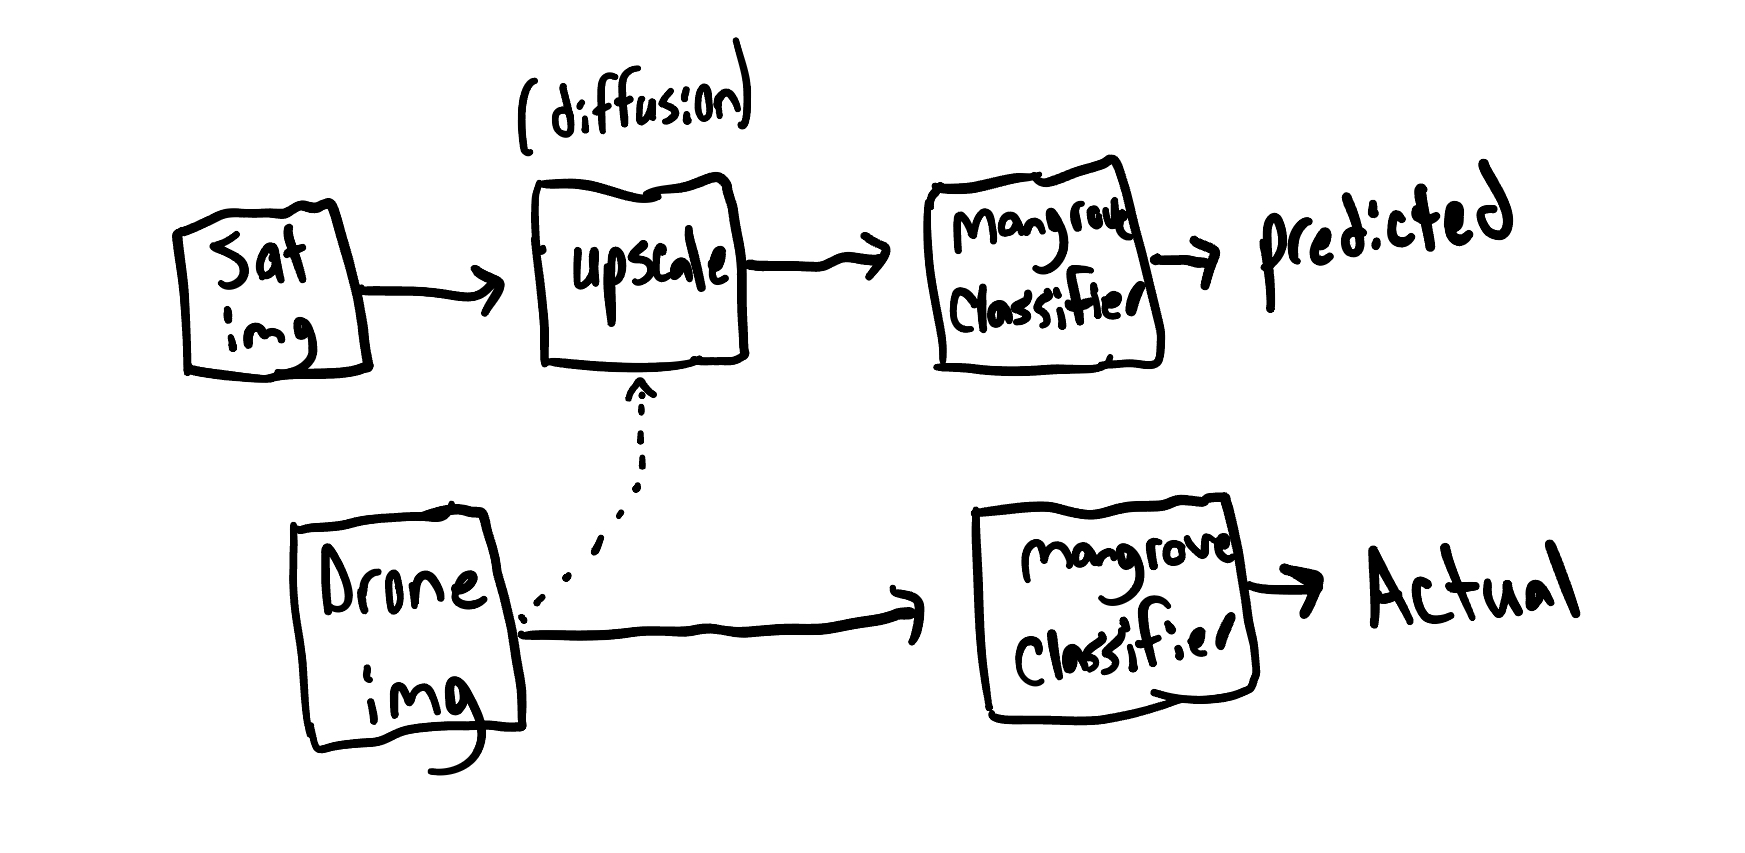
\includegraphics[height=0.7\textheight,width=0.7\textwidth,keepaspectratio]{images/superres.jpeg}
\end{frame}

% To create a slide with a bullet list, use the following:
% \begin{frame}{TITLE}
%     \begin{itemize}
%         \item ITEM 1
%         \item ITEM 2
%     \end{itemize}    
% \end{frame}

% To create a slide with numbered list, use the following:
% \begin{frame}{TITLE}
%     \begin{enumerate}
%         \item ITEM 1
%         \item ITEM 2
%     \end{enumerate}
% \end{frame}

% To create a slide with a graphic:
% 1. Add the graphic to this folder (named picture.png)
% 2. Use the following:
% \begin{frame}{TITLE}
%     \centering
%     \includegraphics[height=0.7\textheight,width=0.7\textwidth,keepaspectratio]{picture.png}
% \end{frame}

% To create a slide with two columns, use the following:
% \begin{frame}{TITLE}
%     \begin{columns}
%         \begin{column}{0.5\textwidth}
%             COLUMN 1 BODY
%         \end{column}
%         \begin{column}{0.5\textwidth}
%             COLUMN 2 BODY
%         \end{column}
%     \end{columns}
% \end{frame}
